\documentclass[tikz,border=5pt]{standalone}
\usepackage{tikz}
\usetikzlibrary{math}

\tikzset{
	gurantee/.style={draw, circle, minimum size=22mm},
	every path/.style={color=gray}
}

\begin{document}
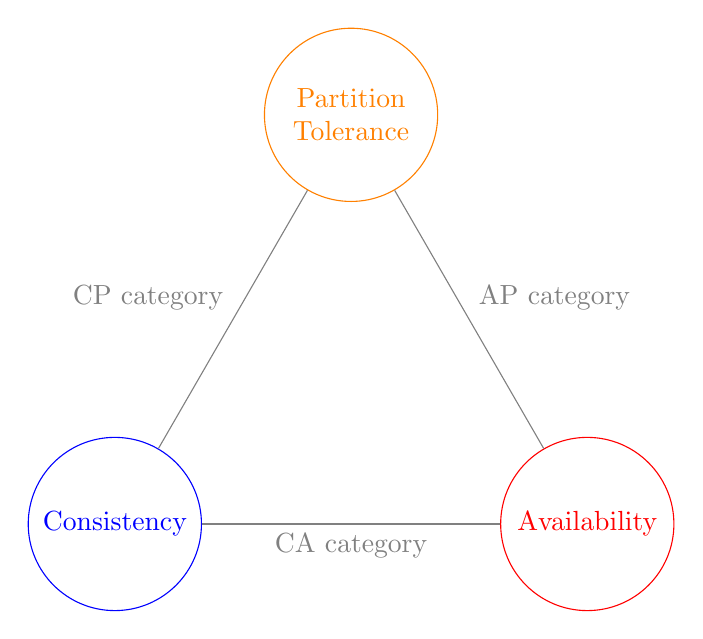
\begin{tikzpicture}
	\tikzmath{\a = 3;}
	\node[gurantee, color=blue]                 (C) at (0, 0)               {Consistency};
	\node[gurantee, color=red]                  (A) at ({2 * \a}, 0)        {Availability};
	\node[gurantee, color=orange, align=center] (P) at (\a, {sqrt(3) * \a}) {Partition\\Tolerance};

	\draw (C) -- (A) node[midway, below]       (CA) {CA category};
	\draw (A) -- (P) node[midway, above right] (AP) {AP category};
	\draw (P) -- (C) node[midway, above left]  (CP) {CP category};
\end{tikzpicture}
\end{document}
